To accomplish the goals 

This chapter will illuminate the details of how encryption, authentication, network coding, and ARQ management are implemented in the network
interfaces.

Recall that the architecture of a \gls{noc} consists of a router grid with each node connected to a local processing element through a network
interface (cf. Figure \vref{fig:nocexample}). The 

Over the course of this chapter, the design of the communication protocol in all variants will be thorougly explained. To begin, fundamental
assumptions about the environment and basic building blocks of the protocol are presented. Since the protocol variants share many elements and differ
mostly in the authentication scheme, the simplest one (uncoded individual authentication) is used to give a step-by-step explanation of the full
protocol. Following this, the other variants are described by drawing upon the differences to uncoded individual authentication.

\section{Design Considerations}
\subsection{Flit Structure}
As mentioned in Section \ref{sec:flitsfun}, flits are the fundamental unit of transmission for this thesis. They contain several header fields and a
payload. Their structure differs slightly depending on whether or not network coding is employed. In a network coded environment, one additional
header field is required (the global encoding vector) and the generation ID replaces the flit ID. This structure is depicted in Figure
\vref{fig:flitstructureuncoded} (uncoded) and Figure \ref{fig:flitstructurenetworkcoded} (network coded).
% TODO: table comparing the protocol variants, their properties (e.g. lane width)

\begin{figure}
    \centering
    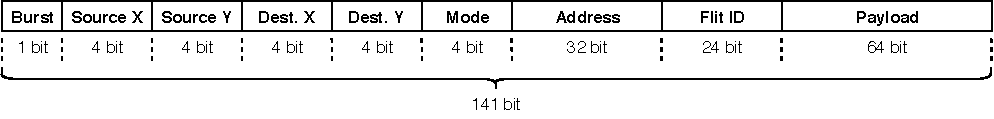
\includegraphics[width=\textwidth]{flit-structure-uc}
    \caption[The structure of a flit without network coding]{The structure and data layout of a flit in an environment without network coding
    (uncoded). The fixed size of the header fields and the payload results in an invariant total size of 141 bit.}
    \label{fig:flitstructureuncoded}
\end{figure}

\begin{figure}
    \centering
    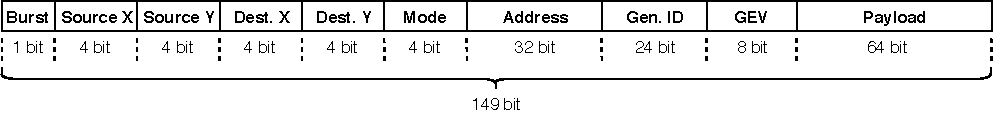
\includegraphics[width=\textwidth]{flit-structure-nc}
    \caption[The structure of a flit with network coding]{The structure and data layout of a flit in a network coded environment. The fixed size of
    the header fields and the payload results in an invariant total size of 149 bit.}
    \label{fig:flitstructurenetworkcoded}
\end{figure}

The header fields are required for routing the flits to their destinations and for correct processing by the receivers, while the payload carries the
transmitted information. Uncoded flits have the following fields:
\begin{itemize}
    \item \textbf{Burst.} The burst bit is used to indicate an uninterrupted stream of flits between the same sender and receiver. For example, when a
        larger packet is being broken down into multiple flits, the burst bit can be used to indicate the beginning of a flit stream, allowing the
        intermediate routers on the path to the receiver to adjust their routing behavior accordingly in order to minimize stream interruptions. In
        this thesis, however, the burst bit is unused. As there are plans to build upon this work and explore burst configurations, it is still
        included for documentation purposes.
    \item \textbf{Source X, Source Y.} Recalling that the topology of the \gls{noc} is a 2D mesh, the usage of 2D cartesian coordinates to uniquely
        identify nodes suggested itself. Here, zero-based X and Y indices indicate the column and row of a node, respectively. Each field is 4 bit long,
        resulting in at most $16 \cdot 16 = 256$ nodes being addressable. Hence, the maximum \gls{noc} size is \textit{16x16} as well, which is deemed
        sufficient\footnote{It is certainly possible to increase the field sizes to, e.g., 8 bit, allowing for up to $256 \cdot 256 = 65536$ addressable
        nodes, should the need arise. However, as this would increase the flit size, it is not implemented here.}. The source header fields describe
        the address of the flit's sender.
    \item \textbf{Destination X, Destination Y.} These fields also describe the address of a node in 2D cartesian coordinates. As opposed to the
        source fields, they indicate the intended destination of the flit.
    \item \textbf{Mode.} The mode field indicates what type of data the flit contains. It signals to the receiver whether the flit contains, e.g.,
        encrypted data, a \gls{mac}, or an \gls{arq}. There are a few more special modes that are explained in Section \ref{sec:theprotocol}. The
        field size is 4 bit, allowing for 16 different modes. Not all of them are used for this thesis, so it is possible to define additional modes
        in a future work if necessary.
    \item \textbf{Address.} This field may contain a 32 bit memory address. In case the flit payload needs to be read from or written to memory, it
        indicates the location of the data. Since this is only relevant to the processing elements and not the network interfaces, the field remains
        unused for this thesis. Nevertheless, it is included in the flits since it affects their size.
    \item \textbf{Flit ID.} The flit ID is a 24 bit numeric identifier. Starting at zero, the IDs are incremented as more flits are generated.
        Similar to sequence numbers (e.g., as employed in \gls{tcp}), they are used to ensure that all flits arrive at the destined processing
        elements in order. Furthermore, it is used to associate related flits. For instance, an encrypted data flit and the corresponding \gls{mac}
        flit have the same ID to express their correlation.
    \item \textbf{Payload.} The payload carries the actual data that are transmitted with a flit. Its size is 64 bit as this is a common plaintext
        size for block ciphers, such as the one used for this thesis, PRINCE \cite{borghoff12prince}.
\end{itemize}

When network coding is employed, the following fields are added:
\begin{itemize}
    \item \textbf{Generation ID.} Replacing the flit ID, the generation ID is also a 24 bit numeric idenfier. As network coding intermingles multiple
        flits, their original IDs become meaningless and are replaced by the generation ID (which is the same for all flits of a generation). Apart
        from this, they follow the same rules as the flit IDs described above.
    \item \textbf{Global Encoding Vector.} This field contains the global encoding vector used to create the flit when applying network coding. It is
        required for the receiver to successfully decode a generation and obtain the original flits. Furthermore, since all flits in a generation have
        the same ID, it is used to distinguish between those flits. As with flit IDs in an uncoded setting, corresponding flits (like data and
        \gls{mac}) are associated by having the same \gls{gev} in addition to the same generation ID.
\end{itemize}

Flits can be transferred in a single clock
cycle between directly connected components. For example, sending a flit from one router to a neighboring one, or sending it from a processing element
to the corresponding network interface takes one cycle. In a hardware implementation, this is facilitated by parallel communication channels that can
transmit multiple bits simultaneously. At the physical layer, this results in multiple wires (or other electical conductors), as each one may convey
precisely one bit of information \cite{wikiparallelcomm}. Thus, for uncoded flits, a channel width of 141 or more wires is required, and at least 149
in a network coded setting.

% TODO: where to put the following paragraph?
For each sender-receiver pair, a
flit's ID must be unique when it is generated by the sending processing element\footnote{As the maximum possible value of a 24 bit number is
$2^{24}-1$, long-running systems are bound to cause an arithmetic overflow at some point. If this happens, IDs are allowed to repeat themselves,
restarting at zero.}. 

\subsection{ARQ Structure}

\subsection{Network Coding}\label{sec:designnc}
The coding scheme used in this work slightly differs from the one described above. First, it is applied to unicast transmissions, while traditional
network coding focuses on multicast scenarios \cites{ahlswede00networkflow}{li03linearnc}. Second, only the sender nodes will compute combinations of
different flits, while intermediate nodes merely forward them. The rationale behind this are the tight performance requirements of \glspl{noc}. If
each network node waited for enough flits to perform local encoding before forwarding, routing latencies would increase. Furthermore, the
implementation of local encoding implies additional logic in each router, making their design more complex and entailing a higher chip area
requirement. However, this directly contradicts the \gls{noc} design goals laid out in Section \ref{sec:networkonchipfun} and is thus not considered.
% Only the sender codes
% TODO: mention PNC paper, that we use RLNC, but only senders encode and create generations ("only intra-session network coding")
% TODO: a bit of math and formulas on how NC is done (inspired by previous TUD papers)
% 2 sub-variants: G2C3, G2C4
% Why G2C3 and G2C4? → refer to previous TUD papers

\section{The Protocol}\label{sec:theprotocol}
As mentioned in Section \ref{sec:protocolvariants}, three different communication schemes were envisioned, with the first two subdivided into uncoded
and network coded versions. The remainder of this section provides a comprehensive specification of all variants.

\subsection{Individual Authentication}
\begin{figure}
    \centering
    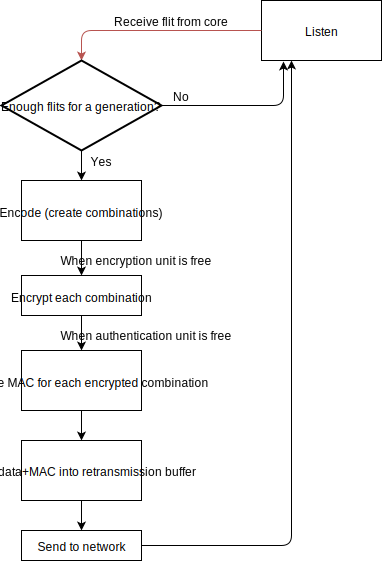
\includegraphics[width=\textwidth]{protocol-flowchart-nc-1}
    \caption[Protocol flow: method 1 coded]{Protocol flow: method 1 coded}
    \label{fig:protchartnc1}
\end{figure}
% uncoded (full explanation), network coded

\subsection{Interwoven Authentication}

\subsection{Full-Generation Authentication}

\section{Routing Strategies}
Mention the perceived/envisioned advantages of adaptive routing (different paths for each flit within the same sender-receiver pair → thanks
to NC enough flits will arrive hopefully even if one path contains a corrupted router).

\subsection{Deterministic XY}
The term \enquote{XY routing} stems directly from the behavior of the routers: flits are only routed along the X axis until they arrive in the column
that the receiver lies in, at which they are routed along the Y axis until reaching the receiver node.
% TODO: figure with a 2D mesh, X and Y arrows on the sides, example path marked for a transmission
\subsection{Dynamic Smart Random}
\subsection{Randomized Oblivious Multi-phase Minimal}
% Both with XY phases and DSR phases
This strategy essentially splits the routing problem into two phases: find a path from sender to proxy node and from proxy to receiver. For each
phase, one of the aforementioned strategies can be applied as is.

\begin{itemize}
    \item Routing Strategies
        \begin{itemize}
            \item Mention routing is general, we are special case of 2D mesh with uniform edge weights → much simpler than arbitrary networks
            \item XY/YX
                \begin{itemize}
                    \item Deterministic path
                    \item Attacker controlling a single router can reliably disrupt communication between certain nodes
                    \item does not distribute flits of a generation across different paths
                \end{itemize}
            \item XY/YX + Valiant
                \begin{itemize}
                    \item Deterministic path only if fixed valiant
                \end{itemize}
            \item Random XorY
            \item Random XorY + Valiant
            \item When writing about this: MANHATTAN DISTANCE (same for XY, YX, random XY, ROMM)
            \item Terminology:
                \begin{itemize}
                    \item Static=deterministic vs. dynamic (one fixed source-destination route or not)
                    \item Oblivious vs. adaptive (take into account network state or not)
                    \item Source routing: source decides a path, this is inserted into flit as metadata
                    \item ROMM is oblivious, use own term RAMM (randomized adaptive multi-phase minimal) for other variant
                    \item ROMM: oblivious, dynamic
                    \item DOR (dimension order routing): oblivious, deterministic
                \end{itemize}
        \end{itemize}
\end{itemize}

\iffalse
\section{Notes}
\begin{itemize}
    \item Encryption/authentication ordering
        \begin{itemize}
            \item Encrypt-then-MAC: best practice. Sequential encrypt/authenticate on sender side, but parallel decrypt/verify
                on receiver side. Advantage: MAC can be computed on receiver side immediately when ciphertext arrives, even when
                MAC flit has not arrived yet (if ARQ is necessary, it can be issued right away)
            \item MAC-then-encrypt: bad. Sequential authenticate/encrypt on sender side and sequential decrypt/verify on receiver
                side.
            \item Encrypt-and-MAC: okay. Parallel encrypt/authenticate on sender side, but sequential decrypt/verify on receiver
                side (overall same latency as Encrypt-then-MAC, but without advantage of fast ARQs)
        \end{itemize}
    \item Uncoded transmission
        \begin{itemize}
            \item no network coding
            \item 2 methods: 1 data flit + 1 MAC flit OR 2 data/MAC split flits
        \end{itemize}
    \item Flit structure
        \begin{itemize}
            \item burst bit, source/target address, mode, address, GID/FID, GEV, payload
            \item mode: define if data/mac/split/arq
        \end{itemize}
    \item Network coded transmission
        \begin{itemize}
            \item Number of flits: G2C3 or G2C4
            \item 3 methods: 1 data flit + 1 MAC flit OR 1 MAC flit per generation OR 2 data/MAC split flits
            \item mention that coded clits are slightly larger due to GEV being embedded → requires wider lanes
        \end{itemize}
    \item ARQs
        \begin{itemize}
            \item Limited number of ARQs per transmission unit (UC: data/MAC pair or split pair, NC: generation)
            \item Timeout of x (e.g. 8) cycles until first ARQ is sent
            \item If limit >1: start larger timeout (→ round-trip of ARQ)
            \item Many different cases, insert some flow diagrams here
            \item The higher the ARQ timeout/limit, the less likely the flit is still in retransmission buffer
            \item → ARQ timeout/limit and retransmission buffer size have to correlate
            \item In the case that we only have 1 ARQ left that we are allowed to send: Wait for any ongoing MAC verifications
                so in case they fail, the flits can be included in the ARQ
        \end{itemize}
\end{itemize}
\fi
